\documentclass[11pt]{article}
\title{\textbf{Meccano octagons}}
\author{https://github.com/heptagons/meccano/octa}
\date{}

\usepackage{amsmath}
\usepackage{listings}
\usepackage{xcolor}
\definecolor{gray}{RGB}{245,245,245}

\lstset{
	backgroundcolor=\color{gray},
	frame=single,
	numbers=left,
	stepnumber=1,
	tabsize=4,
	basicstyle=\ttfamily\small,
	breaklines=true
}

\usepackage[margin=0.75in]{geometry}

\usepackage{tikz}
\usetikzlibrary{math}

\usepackage{graphicx}

\begin{document}

\maketitle

\newcommand{\rod}[4][000000] % [color]{n}{sep}{prop}
{
 \definecolor{main}{HTML}{#1}
 \draw[main] (0,{{2*#4}})
   -- ++({#2*#3},0) arc(+90:-90:{2*#4})
   -- ++({-#2*#3},0) arc(270:90:{2*#4});
 \foreach \x in {0,1,...,#2}
  \draw[main] (\x*#3,0) circle (#4);
}

\section{Meccano regular octagons}

\begin{figure}
\centering
\scalebox{0.8}{
 \begin{tikzpicture}
 \def\p{3pt}
 \begin{scope}[rotate=-90]
  \draw[dash dot] (0,0) -- (6,6);
  \begin{scope}[rotate=64.5]
   \rod[FF3300]{9}{1}{\p} % ADn
   \end{scope}
   \rod{6}{1}{\p} % AB
   \path (0,0) ++(222:5*\p) node{A};
   \begin{scope}[shift={(6,0)},rotate=90]
    \rod[009900]{6}{1}{\p} % BC
    \path (0,0) ++(222:5*\p) node{B};
    \begin{scope}[shift={(6,0)},rotate=45]
     \rod[009900]{6}{1}{\p} % CE
     \path (0,0) ++(222:5*\p) node{C};
     \path (1,0) ++(-90:5*\p) node{$D_1$};
     \path (2,0) ++(-90:5*\p) node{$D_2$};
     \path (3,0) ++(-90:5*\p) node{$D_n$};
     \path (4,0) ++(-90:5*\p) node{...};
     \path (6,0) ++(-75:5*\p) node{E};
    \end{scope}
   \end{scope}
   \begin{scope}[shift={(2,0)},rotate=37] %FG
    \rod[0033FF]{5}{1}{\p}
    \path (0,0) ++(75:5*\p) node{F};
    \path (5,0) ++(115:5*\p) node{G};
   \end{scope}
  \end{scope}
 \end{tikzpicture}
}
\caption{plan}
\label{fig:plan}
\end{figure}


Meccano regular octagons are build with eight equals rods to form the perimeter and several
extra rods as internal diagonals to make rigid the octagon's internal angles equal to $135^\circ{}$. 
Figure \ref{fig:plan} show the internal diagonals construction. The idea is to form two adjacent
triangles with two angles adding to $145^\circ{}$. Consider triangle $ABC$ with
$\angle{BCA} = 45^\circ{}$ and triangle $ACD_n$ with $\angle{ACD_n} = 90^\circ{}$,
so $\angle{BCE} = 135^\circ{}$. Lets define:
\begin{align*}
a &= \overline{AD_n}\\
b &= \overline{CD_n}\\
c &= \overline{AB} = \overline{BC} = \overline{CE}
\end{align*}

The internal diagonal we are looking for is the integer $a$ (shown in red) and the two
adjacent octagon sides are $c = \overline{BC} = \overline{CE}$ (shown in green).
The common hyphotenuse shown in the figure as a dashed line value is $\overline{AC} = \sqrt{2}c$ so:
\begin{align*}
(\sqrt{2}c)^2 &= a^2 - b^2\\
         2c^2 &= a^2 - b^2\\
            c &= \sqrt{\frac{a^2 - b^2}{2}}
\end{align*}

We need a program to test pairs $a > b$ which makes a $c$ an integer too.

\subsection{Octagons diagonals program}

Next golang listing program finds valid octagons diagonals $a$ and sides $\max(b,c)$.
First we iterate diagonals from 1 to a given maximum (line 2).
Then we iterate over integer $b$ from $1$ to $a$ (line 3).
We calculate $2c^2$ and check if its even (lines 4, 5) and the we check
if $c$ is an integer (line 8). To prevent repetitions by scaling we check
the greatest common divisor to be 1 (line 9) and print a valid result 
where the octagon size is the maximum value of $b$ or $c$. (line 11).
\begin{lstlisting}
func octagons_2(max int) {
	for a := 1; a < max; a++ {
		for b := 1; b < a; b++ {
			cc := a*a - b*b
			if cc % 2 == 0 {
				f := math.Sqrt(float64(cc/2))
				c := int(f)
				if f == float64(c) {
					if gcd(c, gcd(b, a)) == 1 {
						s := int(math.Max(float64(b), f))
						fmt.Printf("a=%2d b=%2d c=%2d s=%2d\n", a, b, c, s)
					}
				}
			}
		}
	}
}

func gcd(a, b int) int { // greatest common divisor
	if b == 0 {
		return a
	}
	return gcd(b, a % b)
}
\end{lstlisting}

\subsection{Octagons diagonals results}

Program's first results are shown in the next listing.
Important integers are $a$ the diagonal and $s$ the size.
\begin{lstlisting}
a= 3 b= 1 c= 2 s= 2
a= 9 b= 7 c= 4 s= 7
a=11 b= 7 c= 6 s= 7
a=17 b= 1 c=12 s=12
a=19 b=17 c= 6 s=17
a=27 b=23 c=10 s=23
a=33 b=17 c=20 s=20
a=33 b=31 c= 8 s=31
a=41 b=23 c=24 s=24
a=43 b= 7 c=30 s=30
a=51 b=47 c=14 s=47
a=51 b=49 c=10 s=49
a=57 b= 7 c=40 s=40
a=57 b=41 c=28 s=41
a=59 b=41 c=30 s=41
\end{lstlisting}

\newcommand{\fixer}[6] %{f}{p}{s}{d}{angle}{extra}
{
 \begin{scope}[shift={(#1*#6,0)}]
  \begin{scope}[rotate=90]
   \rod[000000]{#3}{#1}{#2}
   \begin{scope}[shift={(4*#1,0)},rotate=-143]
    \rod[0033FF]{5}{#1}{#2}
   \end{scope} 
   \begin{scope}[shift={(#1*#3,0)},rotate=-135+#5]
    \rod[FF3300]{#4}{#1}{#2}
   \end{scope} 
  \end{scope}
 \end{scope}
}

\newcommand{\octagon}[6] %{f}{p}{s}{d}{angle}{extra}
{
 \begin{tikzpicture}
  \pgfmathsetmacro{\s}{#3+#6}
  \begin{scope}
   \rod[009900]{\s}{#1}{#2} \path (0,0) ++(240:5*#2) node{A};
   \fixer{#1}{#2}{#3}{#4}{#5}{#6}
   \begin{scope}[shift={(\s*#1,0)},rotate=45]
    \rod[009900]{\s}{#1}{#2} \path (0,0) ++(240:5*#2) node{B};
    \fixer{#1}{#2}{#3}{#4}{#5}{#6}
    \begin{scope}[shift={(\s*#1,0)},rotate=45]
     \rod[009900]{\s}{#1}{#2} \path (0,0) ++(240:5*#2) node{C};
     \fixer{#1}{#2}{#3}{#4}{#5}{#6}
     \begin{scope}[shift={(\s*#1,0)},rotate=45]
      \rod[009900]{\s}{#1}{#2} \path (0,0) ++(240:5*#2) node{D};
      \fixer{#1}{#2}{#3}{#4}{#5}{#6}
      \begin{scope}[shift={(\s*#1,0)},rotate=45]
       \rod[009900]{\s}{#1}{#2} \path (0,0) ++(240:5*#2) node{E};
       \fixer{#1}{#2}{#3}{#4}{#5}{#6}
       \begin{scope}[shift={(\s*#1,0)},rotate=45]
        \rod[009900]{\s}{#1}{#2} \path (0,0) ++(240:5*#2) node{F};
        \begin{scope}[shift={(\s*#1,0)},rotate=45]
         \rod[009900]{\s}{#1}{#2} \path (0,0) ++(240:5*#2) node{G};
         \begin{scope}[shift={(\s*#1,0)},rotate=45]
          \rod[009900]{\s}{#1}{#2} \path (0,0) ++(240:5*#2) node{H};
         \end{scope}
        \end{scope}
       \end{scope}
      \end{scope}
     \end{scope}
    \end{scope}
   \end{scope}
  \end{scope}
 \end{tikzpicture}
}

\begin{figure}
\centering
\scalebox{0.5}{
 \octagon{2}{3pt}{4}{6}{19.5}{0}
}
\caption{The smallest octagon with diagonals $6$ and sides $4$.}
\label{fig:smallest}
\end{figure}

\begin{figure}
\centering
\scalebox{0.5}{
 \octagon{1.4}{3pt}{4}{6}{19.5}{1}
}
\caption{Octagon with diagonals $6$ and sides $5$.}
\label{fig:second}
\end{figure}

\begin{figure}
\centering
\scalebox{1}{
 \octagon{0.5}{3pt}{4}{6}{19.5}{2}
}
\caption{Octagon with diagonals $6$ and sides $6$.}
\label{fig:third}
\end{figure}

\begin{figure}
\centering
\scalebox{1}{
 \octagon{0.5}{3pt}{4}{6}{19.5}{3}
}
\caption{Octagon with diagonals $6$ and sides $7$.}
\label{fig:fourth}
\end{figure}

\begin{figure}[htpb]
\centering
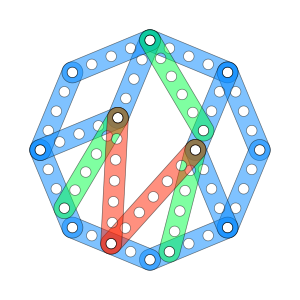
\includegraphics[]{figs/octagon-4}
\caption{The smallest octagon with sides $4$ and with fewest diagonals.}
\label{fig:smallest-simpler}
\end{figure}

\subsection{Octagons with diagonal=$6$}

We can't use the first result $a=3$, $b=1$, $c=2$ and $s=2$ since $s$ is to small. To make rigid the angle of $90^\circ{}$ of triangle $ABC$ in figure \ref{fig:plan} we need a rod of size $5$ at least, as shown the points $F$ and $G$ of the figure.
Scaling by $2$ the first result we have a diagonal $a=6$ and size=$4$ 
as a base to build the smaller octagons.

Figure \ref{fig:smallest} is the smallest octagon; we need to scale the bars in order
the bolts don't collapse with others, the complexity of bars can be simplified 
symmetrically as is show in figure \ref{fig:smallest-simpler}.
In figure \ref{fig:second} we increase the side from $4$ to $5$ but keeping the same diagonal of $6$. In figure \ref{fig:third} we increase the side to $6$ and in figure
\ref{fig:fourth} the side is increased to $7$.


\subsection{Octagons with diagonal=$9$}

\begin{figure}
\centering
\scalebox{0.5}{
 \octagon{0.75}{3pt}{4}{9}{51}{3}
}
\caption{Octagon with diagonal $9$ and side $7$.}
\label{fig:9-7}
\end{figure}

\begin{figure}
\centering
\scalebox{0.5}{
 \octagon{0.5}{3pt}{4}{9}{51}{4}
}
\caption{Octagon with diagonal $9$ and side $8$.}
\label{fig:9-8}
\end{figure}


\begin{figure}
\centering
\scalebox{0.5}{
 \octagon{0.5}{3pt}{4}{9}{51}{5}
}
\caption{Octagon with diagonal $9$ and side $9$.}
\label{fig:9-9}
\end{figure}

\begin{figure}
\centering
\scalebox{0.6}{
 \octagon{0.5}{3pt}{4}{9}{51}{6}
}
\caption{Octagon with diagonal $9$ and side $10$.}
\label{fig:9-10}
\end{figure}

\begin{figure}
\centering
\scalebox{0.6}{
 \octagon{0.5}{3pt}{4}{9}{51}{7}
}
\caption{Octagon with diagonal $9$ and side $11$.}
\label{fig:9-11}
\end{figure}

Using the second result $a=9$, $b=7$, $c=4$ and $s=7$ we form a second group
of octagons. Figure \ref{fig:9-7} shows the smallest octagon with diagonals $9$
and sides $7$. Figures \ref{fig:9-8}, \ref{fig:9-9}, \ref{fig:9-10} and \ref{fig:9-11} show octagons with diagonals $9$ with sides of $8$, $9$, $10$ and $11$.

\subsection{Octagon with two diagonals}

\begin{figure}
\centering
\scalebox{0.8}{
 \begin{tikzpicture}
   \begin{scope}
    \def\f{1} \def\p{3pt}
    \rod[009900]{7}{\f}{\p}
    \path (0,0) ++(222:5*\p) node{A};
    \begin{scope}[shift={(7*\f,0)},rotate=45]
     \rod[009900]{7}{\f}{\p}
     \path (0,0) ++(222:5*\p) node{B};
     \path (7,0) ++(0:5*\p) node{C};
    \end{scope}
    \begin{scope}[shift={(3*\f,0)},rotate=90]   
     \rod{4}{\f}{\p}
     \path (0,0) ++(180:5*\p) node{D};
     \path (4,0) ++(60:5*\p) node{E};
     \begin{scope}[shift={(4*\f,0)},rotate=-135+19.5]
      \rod[FF3300]{6}{\f}{\p}
      \path (6,0) ++(0:5*\p) node{F};
     \end{scope}
     \begin{scope}[shift={(4*\f,0)},rotate=-135+51]
      \rod[FF3300]{9}{\f}{\p}
      \path (9,0) ++(-30:5*\p) node{G};
     \end{scope}
     
    \end{scope}
   \end{scope}
 \end{tikzpicture}
}
\caption{Octagon angle $ABC$ fixed with two diagonals.
The union of rods $\overline{BG}$, $\overline{EF}$ and $\overline{EG}$ is rigid.
Adding two rods $\overline{AB}$ and $\overline{DE}$ remains rigid.}
\vspace{128in} %push to top
\label{fig:diags2}
\end{figure}

By comparing figures \ref{fig:fourth} and \ref{fig:9-10} both with sides=$7$ we can 
make use of two diagonals at the same time and omit the rod $FG$ of figure \ref{fig:plan} used until now to make the $90^\circ{}$ angle. Figure \ref{fig:diags2} show a
octagon angle with two diagonals. In other words, for two results or their scaling,
when both have the same $c$, we can use the two diagonals an omit the $5$ rod.

\end{document}